% En esta seccion se presentan algoritmos, diagramas de flujo, diagramas de arquitecturas del programa, así como requerimientos de hardware y software. Presenta segmentos de código relevantes, figuras ilustrativas debidamente tituladas y referenciadas en el texto.

\section{Metodología de la práctica}

\subsection{Requerimientos de hardware y software}
La práctica se desarrolló sobre el proyecto base proporcionado por el profesor,
que se compila como una aplicación de escritorio de C++ enlazada contra OpenGL.
En la Tabla \ref{tab:requerimientos} se resumen los recursos que se emplearon;
todos ellos cumplen con lo indicado en el manual de la práctica, que pide
Windows 10 o Linux y Visual Studio 2017 o superior \cite{teodoro_manual03}.

\begin{table}[H]
\centering
\begin{tabular}{@{}p{4.0cm}p{10.5cm}@{}}
\toprule
\textbf{Elemento} & \textbf{Especificación empleada} \\
\midrule
Sistema operativo & Windows 11 (64 bits) \\
Entorno de desarrollo & Microsoft Visual Studio, conjunto de herramientas MSVC, plataforma x64 \\
Lenguaje & C++ (estándar \texttt{c++20}) \\
API gráfica & OpenGL 3.3, perfil \textit{core} \\
Bibliotecas & GLFW (creación de la ventana y manejo de eventos), GLAD (carga de las funciones de OpenGL) y GLM (álgebra de vectores y matrices) \\
Hardware & Equipo de cómputo con adaptador gráfico, integrado o dedicado, compatible con OpenGL 3.3 \\
Archivos de apoyo & \texttt{shaders/02-simplePVM.vs} y \texttt{shaders/02-simplePVM.fs}, ubicados en el directorio de trabajo del ejecutable \\
\bottomrule
\end{tabular}
\caption{Requerimientos de hardware y software utilizados en la práctica.}
\label{tab:requerimientos}
\end{table}

La configuración del proyecto siguió los mismos pasos de la práctica anterior:
se creó una carpeta de proyecto dentro de \texttt{03\_GeomModelling}, se agregó
el archivo de origen, se fijó el directorio de salida y el de trabajo en
\texttt{bin}, y se declararon los directorios de inclusión
(\texttt{deps/glad}, \texttt{deps/glfw}, \texttt{deps/glm} y el directorio
\texttt{include} de la práctica), los directorios de bibliotecas y las entradas
del vinculador (\texttt{opengl32.lib}, \texttt{glad.lib} y \texttt{glfw3.lib}).
El directorio de trabajo es indispensable porque los shaders se cargan con una
ruta relativa. Se reutilizaron los shaders \texttt{02-simplePVM.vs} y
\texttt{02-simplePVM.fs} de la práctica anterior, ya que la cadena de
transformaciones no cambia en esta práctica.

\subsection{Arquitectura del programa y flujo de ejecución}
El programa conserva la organización del proyecto base: la función
\texttt{Start()} se ejecuta una sola vez y prepara la ventana, el contexto de
OpenGL, los shaders y las geometrías, mientras que \texttt{Update()} se ejecuta
una vez por cuadro y se encarga de leer el teclado, armar las matrices y
dibujar. En la Figura \ref{fig:flujo} se muestra el flujo completo. Al igual
que en la práctica anterior, la lectura del teclado ocurre \emph{antes} de
construir las matrices, pues de lo contrario la imagen desplegada
correspondería siempre al estado del cuadro anterior.

\begin{figure}[H]
    \centering
    
\includegraphics[width=0.60\textwidth]{Imagenes/Diagramas/flujo.png}
    \caption{Diagrama de flujo del programa \texttt{03\_GeomModelling.cpp}.}
    \label{fig:flujo}
\end{figure}

Sobre esa estructura se hicieron tres ajustes de carácter general. El primero
fue interpretar el segundo vector de la cámara como el punto al que se mira y
no como una dirección, que es lo que espera \texttt{glm::lookAt}
\cite{glm_manual}; el proyecto base lo inicializa con $(0,0,-1)$, lo cual
funciona por casualidad porque ese punto queda casi alineado con el origen,
pero deja de funcionar en cuanto la cámara se coloca sobre otro eje. El segundo
fue agregar \texttt{glfwSwapInterval(1)} después de crear el contexto, de modo
que el lazo principal quede acotado a la frecuencia de actualización del
monitor \cite{glfw_window}. El tercero fue sustituir los seis bloques de
dibujo que el proyecto base trae comentados, idénticos entre sí salvo por el
nombre de la malla, por una sola función \texttt{dibujarMalla()} que recibe la
malla y aplica la cadena proyección--vista--modelo; con ello agregar una
primitiva se reduce a una línea en un \texttt{switch}. En el Código
\ref{lst:codigo-dibujo} se muestra esa función junto con el cuerpo de
\texttt{Update()}.

\begin{lstlisting}[language=C, caption={Funcion de dibujo comun a las tres primitivas y cuerpo de Update()}, label=lst:codigo-dibujo]
// Dibuja una malla aplicando la cadena de transformaciones proyeccion-vista-modelo.
void dibujarMalla(Mesh* malla) {
    if (malla == nullptr)
        return;

    glUseProgram(myShader->ID);

    glm::mat4 projection = glm::perspective(glm::radians(45.0f),
                                            (float)screenWidth / (float)screenHeight,
                                            0.1f, 1000.0f);
    myShader->setMat4("projection", projection);

    glm::mat4 view = glm::lookAt(camera.Position, camera.View, camera.Up);
    myShader->setMat4("view", view);

    // Las primitivas ya se construyen centradas en el origen,
    // asi que la matriz de modelo es la identidad.
    glm::mat4 model = glm::mat4(1.0f);
    myShader->setMat4("model", model);

    malla->Draw(*myShader);

    glUseProgram(0);
}

bool Update() {
    keyboardCallback(window);

    glClearColor(bgR, bgG, bgB, bgA);
    glClear(GL_COLOR_BUFFER_BIT | GL_DEPTH_BUFFER_BIT);

    // Los ejes se dibujan siempre en relleno para que sigan siendo visibles
    // cuando la figura esta en modo alambre.
    glPolygonMode(GL_FRONT_AND_BACK, GL_FILL);
    dibujarMalla(meshAxis);

    glPolygonMode(GL_FRONT_AND_BACK, modoAlambre ? GL_LINE : GL_FILL);

    switch (figuraActual) {
        case 1:  dibujarMalla(meshPlane);  break;  // Actividad 1
        case 2:  dibujarMalla(meshCube);   break;  // Actividad 2
        case 3:  dibujarMalla(meshCircle); break;  // Actividad 3
        default: break;
    }

    glPolygonMode(GL_FRONT_AND_BACK, GL_FILL);

    glfwSwapBuffers(window);
    glfwPollEvents();

    return true;
}
\end{lstlisting}

Las tres primitivas de esta entrega comparten un mismo principio de
construcción, resumido en la Figura \ref{fig:primitivas}: la figura se define
en su propio sistema de coordenadas y centrada en el origen, se descompone en
triángulos y se entrega a la clase \texttt{Mesh} como un par de arreglos, uno
de vértices y otro de índices. Lo único que cambia de una figura a otra es la
regla con la que se generan esos arreglos.

\begin{figure}[H]
    \centering
    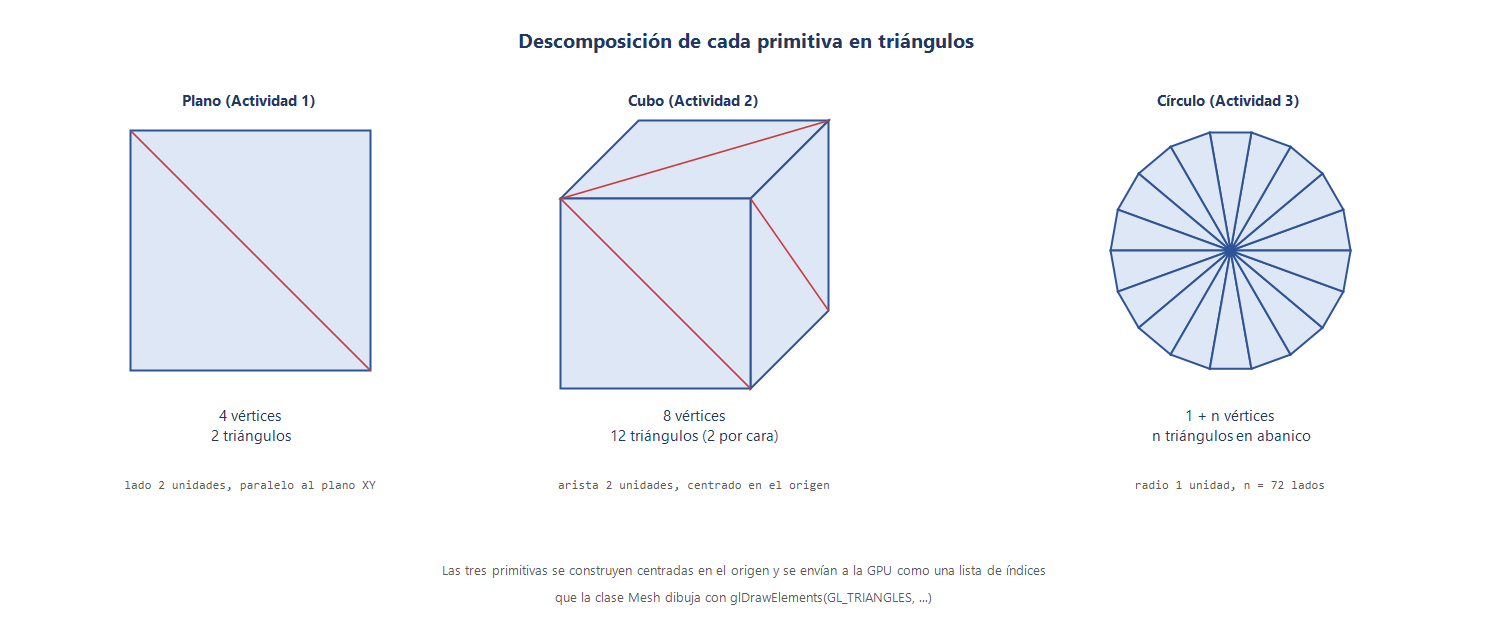
\includegraphics[width=\textwidth]{Imagenes/Diagramas/primitivas.png}
    \caption{Descomposición de las tres primitivas en triángulos, con el número de vértices e índices que genera cada una.}
    \label{fig:primitivas}
\end{figure}

\subsection{Vistas y modo de rasterización}
El manual pide que cada geometría pueda observarse desde dos perspectivas
distintas mediante las teclas \texttt{F1} y \texttt{F2}. Como en esta práctica
la cámara no es el objeto de estudio, ambas vistas se resolvieron reasignando
los tres vectores que recibe \texttt{glm::lookAt}: \texttt{F1} coloca al
observador sobre el eje $+Z$, a cinco unidades del origen, con lo que se
obtiene la vista frontal, y \texttt{F2} lo coloca en el punto $(3,3,3)$, sobre
la diagonal del primer octante, con lo que se obtiene la vista oblicua. En
ambos casos el punto observado es el origen y el vector de orientación es
$(0,1,0)$.

Se agregó además la tecla \texttt{L}, que alterna el modo de rasterización
entre relleno y alambre con \texttt{glPolygonMode}
\cite{khronos_polygonmode}. Esta tecla no la pide el manual, pero resultó
indispensable para las tres actividades, porque es la única forma de comprobar
a simple vista que la descomposición en triángulos es la que se pretendía: en
modo relleno, un triángulo faltante y un triángulo repetido producen a menudo
la misma imagen. El cambio de modo se detecta por flanco y no por estado, ya
que el teclado se consulta una vez por cuadro y, de otro modo, una sola
pulsación alternaría el modo decenas de veces. En el Código
\ref{lst:codigo-teclado} se muestra el manejo del teclado completo.

\begin{lstlisting}[language=C, caption={Seleccion de figura, vistas F1 y F2 y alternancia del modo de rasterizacion}, label=lst:codigo-teclado]
void keyboardCallback(GLFWwindow* window) {

    if (glfwGetKey(window, GLFW_KEY_ESCAPE) == GLFW_PRESS) {
        glfwSetWindowShouldClose(window, true);
    }

    // Seleccion de la primitiva que se despliega
    if (glfwGetKey(window, GLFW_KEY_1) == GLFW_PRESS) {
        figuraActual = 1;   // Actividad 1: plano
    }
    if (glfwGetKey(window, GLFW_KEY_2) == GLFW_PRESS) {
        figuraActual = 2;   // Actividad 2: cubo
    }
    if (glfwGetKey(window, GLFW_KEY_3) == GLFW_PRESS) {
        figuraActual = 3;   // Actividad 3: circulo
    }

    // Alternancia entre relleno y alambre. Se detecta el flanco de la tecla
    // porque el teclado se consulta una vez por cuadro y, de lo contrario,
    // el modo cambiaria decenas de veces con una sola pulsacion.
    bool teclaLActual = (glfwGetKey(window, GLFW_KEY_L) == GLFW_PRESS);
    if (teclaLActual && !teclaLPrevia) {
        modoAlambre = !modoAlambre;
    }
    teclaLPrevia = teclaLActual;

    // Vistas solicitadas por la practica
    if (glfwGetKey(window, GLFW_KEY_F1) == GLFW_PRESS) {
        // Vista frontal: observador sobre el eje +Z mirando al origen
        camera.Position = glm::vec3(0.0f, 0.0f, 5.0f);
        camera.View     = glm::vec3(0.0f, 0.0f, 0.0f);
        camera.Up       = glm::vec3(0.0f, 1.0f, 0.0f);
    }
    if (glfwGetKey(window, GLFW_KEY_F2) == GLFW_PRESS) {
        // Vista oblicua: observador sobre la diagonal del primer octante
        camera.Position = glm::vec3(3.0f, 3.0f, 3.0f);
        camera.View     = glm::vec3(0.0f, 0.0f, 0.0f);
        camera.Up       = glm::vec3(0.0f, 1.0f, 0.0f);
    }
}
\end{lstlisting}

\subsection{Actividad 1: Plano paralelo al plano XY}
La clase \texttt{Plane} del proyecto base ya construye un cuadrilátero contenido
en el plano $z=0$ con cuatro vértices y dos triángulos, de modo que la actividad
se reduce a elegir correctamente el argumento del constructor. El punto que
conviene subrayar es que ese constructor no recibe el semilado sino el lado
completo: internamente calcula \texttt{value = size / 2.0f} y coloca los
vértices en $(\pm\texttt{value}, \pm\texttt{value}, 0)$. Para obtener el plano
de $2\times2$ unidades que pide el manual hay que invocarlo entonces con
\texttt{Plane(2.0f)}, y no con \texttt{Plane(1.0f)} como aparece en el ejemplo
comentado del proyecto base, que produce un plano de $1\times1$. Esa división
entre dos es también la que garantiza que la figura quede centrada en el
origen para cualquier tamaño.

Los cuatro vértices llevan colores distintos (rojo, verde, azul y cian), de
manera que la interpolación que realiza la etapa de rasterización produce un
degradado continuo sobre las dos caras triangulares. En el Código
\ref{lst:codigo-plano} se reproduce la construcción de la clase y la línea con
la que se instancia.

\begin{lstlisting}[language=C, caption={Construccion del plano y su instanciacion con lado 2}, label=lst:codigo-plano]
// --- Clase Plane del proyecto base (include/Plane.h) ---
void buildVertices(float size) {
    float value = size / 2.0f;   // el constructor recibe el lado completo

    Vertex v;

    v.Position.x =  value; v.Position.y =  value; v.Position.z = 0.0f;
    v.Color.x = 1.0f; v.Color.y = 0.0f; v.Color.z = 0.0f;
    vertices.push_back(v);

    v.Position.x = -value; v.Position.y =  value; v.Position.z = 0.0f;
    v.Color.x = 0.0f; v.Color.y = 1.0f; v.Color.z = 0.0f;
    vertices.push_back(v);

    v.Position.x = -value; v.Position.y = -value; v.Position.z = 0.0f;
    v.Color.x = 0.0f; v.Color.y = 0.0f; v.Color.z = 1.0f;
    vertices.push_back(v);

    v.Position.x =  value; v.Position.y = -value; v.Position.z = 0.0f;
    v.Color.x = 0.0f; v.Color.y = 1.0f; v.Color.z = 1.0f;
    vertices.push_back(v);
}

void buildIndices() {
    indices.push_back(0); indices.push_back(1); indices.push_back(2);
    indices.push_back(0); indices.push_back(2); indices.push_back(3);
}

// --- Instanciacion en Start() ---
// Plano paralelo al plano XY, de 2x2 unidades, centrado en el origen.
Plane plane(2.0f);
meshPlane = new Mesh(plane.vertices, plane.indices);
\end{lstlisting}

\subsection{Actividad 2: Cubo centrado en el origen}
El cubo sigue el mismo criterio: la clase \texttt{Cube} recibe la arista
completa y coloca los ocho vértices en $(\pm\texttt{value}, \pm\texttt{value},
\pm\texttt{value})$, por lo que el cubo de $2\times2\times2$ unidades se obtiene
con \texttt{Cube(2.0f)}. Los primeros cuatro vértices corresponden a la cara
$z=-1$ y los cuatro restantes a la cara $z=+1$, y las seis caras se arman con
dos triángulos cada una, para un total de doce triángulos y treinta y seis
índices.

Antes de darlo por bueno verificamos que la lista de índices efectivamente
cubriera las seis caras, ya que un cubo al que le falta una cara se ve idéntico
a uno completo mientras no se le gire lo suficiente. La comprobación se hizo
agrupando los índices por caras: los vértices $\{0,1,2,3\}$ forman la cara
trasera, $\{4,5,6,7\}$ la frontal, $\{0,3,4,7\}$ la derecha, $\{1,2,5,6\}$ la
izquierda, $\{0,1,4,5\}$ la superior y $\{2,3,6,7\}$ la inferior; las seis
aparecen en el arreglo. Conviene notar que el sentido de recorrido no es
consistente entre todas ellas, lo cual no afecta el resultado porque en esta
práctica no se activa el descarte de caras traseras, pero sí lo haría en
prácticas posteriores. En el Código \ref{lst:codigo-cubo} se muestra la
construcción de los índices y la instanciación.

\begin{lstlisting}[language=C, caption={Indices por cara del cubo e instanciacion con arista 2}, label=lst:codigo-cubo]
// --- Clase Cube del proyecto base (include/Cube.h) ---
// Vertices 0..3: cara z = -value    Vertices 4..7: cara z = +value
void buildIndices() {
    // Cara trasera  (z = -value)
    indices.push_back(0); indices.push_back(1); indices.push_back(2);
    indices.push_back(0); indices.push_back(2); indices.push_back(3);

    // Cara frontal  (z = +value)
    indices.push_back(4); indices.push_back(5); indices.push_back(6);
    indices.push_back(4); indices.push_back(6); indices.push_back(7);

    // Cara derecha  (x = +value)
    indices.push_back(0); indices.push_back(3); indices.push_back(4);
    indices.push_back(3); indices.push_back(4); indices.push_back(7);

    // Cara izquierda (x = -value)
    indices.push_back(1); indices.push_back(5); indices.push_back(2);
    indices.push_back(2); indices.push_back(5); indices.push_back(6);

    // Cara superior (y = +value)
    indices.push_back(0); indices.push_back(1); indices.push_back(5);
    indices.push_back(0); indices.push_back(4); indices.push_back(5);

    // Cara inferior (y = -value)
    indices.push_back(2); indices.push_back(3); indices.push_back(6);
    indices.push_back(3); indices.push_back(6); indices.push_back(7);
}

// --- Instanciacion en Start() ---
// Cubo de 2x2x2 unidades, centrado en el origen.
Cube cube(2.0f);
meshCube = new Mesh(cube.vertices, cube.indices);
\end{lstlisting}

\subsection{Actividad 3: Círculo de radio unitario}
El círculo es la primera figura de la práctica que no puede escribirse vértice
por vértice, porque su contorno es una curva. Lo que se hace es aproximarlo con
un polígono regular de $n$ lados: se recorre el ángulo $\theta$ en incrementos
de $360^\circ/n$ y en cada paso se evalúa
\[
    x = r\cos\theta, \qquad y = r\sin\theta, \qquad z = 0,
\]
con lo que se obtienen los $n$ vértices del contorno. La superficie se cubre
después con un abanico de triángulos: un único vértice en el centro se une con
cada par de vértices consecutivos del contorno, de modo que hacen falta $n$
triángulos y $1+n$ vértices en total.

La clase \texttt{Circle} del proyecto base sigue esta misma idea, pero al
ejecutarla encontramos tres problemas que se documentan en la sección de
experimentos: sólo asigna color a los vértices correspondientes a
$0^\circ$, $120^\circ$ y $240^\circ$, y deja los demás con el contenido
indeterminado de la estructura \texttt{Vertex}; duplica el vértice del centro
una vez por cada punto del contorno, de modo que emplea $2n$ vértices en lugar
de $1+n$; y su segundo lazo de índices llega a escribir el valor
\texttt{vertices.size()}, que es un índice que no existe dentro del arreglo.

Por esa razón se reescribió la clase conservando su nombre y su interfaz, para
no alterar el resto del programa. El archivo vive en la carpeta de código de la
práctica, junto al archivo \texttt{.cpp}, y como el compilador resuelve
\texttt{\#include "Circle.h"} buscando primero en el directorio del archivo que
lo incluye, esta versión tiene precedencia sobre la del directorio
\texttt{include} sin necesidad de tocar el proyecto base. El constructor recibe
ahora el radio y el número de lados, con valor predeterminado de 72, es decir,
un vértice cada cinco grados. Para el color del contorno se conservaron los
tres tonos del proyecto original (cian en $0^\circ$, magenta en $120^\circ$ y
azul en $240^\circ$), pero interpolados linealmente entre anclas, de manera que
todos los vértices tengan un valor definido. En el Código
\ref{lst:codigo-circulo} se muestra la clase completa.

\begin{lstlisting}[language=C, caption={Clase Circle reescrita como abanico de triangulos}, label=lst:codigo-circulo]
class Circle {
public:
    // radius: radio de la circunferencia.
    // slices: numero de lados del poligono con el que se aproxima.
    Circle(float radius, int slices = 72) {
        if (slices < 3) slices = 3;
        this->slices = slices;
        buildVertices(radius);
        buildIndices();
    }

    vector<Vertex>       vertices;
    vector<unsigned int> indices;

private:
    int slices;

    // Se conservan los tres tonos del proyecto base (cian en 0 grados,
    // magenta en 120 y azul en 240) pero ahora se interpolan para que
    // todos los vertices tengan un valor definido.
    vec4 colorContorno(float grados) {
        const vec3 anclas[3] = {
            vec3(0.0f, 1.0f, 1.0f),   //   0 grados
            vec3(1.0f, 0.0f, 1.0f),   // 120 grados
            vec3(0.0f, 0.0f, 1.0f)    // 240 grados
        };

        float t = grados / 120.0f;      // sector de 120 grados
        int   i = (int)t % 3;           // ancla inicial
        float f = t - (float)((int)t);  // avance dentro del sector

        vec3 c = anclas[i] * (1.0f - f) + anclas[(i + 1) % 3] * f;
        return vec4(c, 1.0f);
    }

    void buildVertices(float radius) {
        Vertex v;

        // Vertice 0: centro del circulo
        v.Position = vec3(0.0f, 0.0f, 0.0f);
        v.Color    = vec4(0.20f, 0.20f, 0.25f, 1.0f);
        vertices.push_back(v);

        // Vertices 1..slices: contorno sobre el plano XY
        float paso = 360.0f / (float)slices;
        for (int i = 0; i < slices; i++) {
            float grados = paso * (float)i;
            float rad    = radians(grados);

            v.Position = vec3(radius * cos(rad), radius * sin(rad), 0.0f);
            v.Color    = colorContorno(grados);
            vertices.push_back(v);
        }
    }

    void buildIndices() {
        // Un triangulo por cada lado del poligono. El operador modulo cierra
        // el circulo uniendo el ultimo vertice del contorno con el primero.
        for (int i = 0; i < slices; i++) {
            indices.push_back(0);
            indices.push_back(1 + i);
            indices.push_back(1 + (i + 1) % slices);
        }
    }
};

// --- Instanciacion en Start() ---
// Circulo de radio 1 unidad, centrado en el origen, con 72 lados.
Circle circle(1.0f, 72);
meshCircle = new Mesh(circle.vertices, circle.indices);
\end{lstlisting}

\subsection{Actividad 4: Cilindro centrado en el origen}

Para esta actividad se construyó un cilindro tridimensional de radio unitario ($r = 1.0$) y altura de dos unidades ($h = 2.0$) centrado en el origen del sistema cartesiano. Al analizar la plantilla base del archivo \texttt{Cylinder.h}, se encontró que el cuerpo se dibujaba acostado a lo largo del eje $Z$, le faltaban las tapas circulares y la mayor parte de los vértices quedaban sin asignación de color.

La metodología consistió en reescribir la clase utilizando parametrización de radio, altura y subdivisiones angulares:
\begin{enumerate}
    \item \textbf{Generación de anillos perimétricos:} Se generaron dos círculos de 72 vértices cada uno sobre planos paralelos al plano $XZ$: el anillo inferior ubicado en $y = -1.0$ y el superior en $y = +1.0$. Las coordenadas horizontales se obtuvieron mediante $x = r \cos(\theta)$ y $z = r \sin(\theta)$ con incrementos angulares regulares.
    \item \textbf{Interpolación de color:} Se aplicó una función de mezcla de colores suave que recorre diferentes tonalidades de azul en función del ángulo $\theta$.
    \item \textbf{Construcción del manto lateral:} Se conectaron los vértices de ambos anillos formando dos triángulos por cada sector angular, asegurando el orden horario y antihorario para la orientación de caras.
    \item \textbf{Cierre de tapas:} Se agregaron dos vértices centrales adicionales: uno en $(0, +1.0, 0)$ para la tapa superior y otro en $(0, -1.0, 0)$ para la inferior. Cada tapa se construyó mediante un abanico de triángulos conectando el centro con cada segmento del perímetro.
\end{enumerate}

El código implementado en la clase \texttt{Cylinder.h} fue:

\begin{lstlisting}[language=C++, caption={Construcción geométrica y tapas del cilindro en Cylinder.h.}]
void buildGeometry(float radius, float height, int sectors) {
    float halfH = height * 0.5f; // Rango de -1.0 a +1.0

    // 1. Anillo inferior (y = -halfH)
    for (int i = 0; i < sectors; ++i) {
        float theta = glm::radians(i * (360.0f / (float)sectors));
        Vertex v;
        v.Position = glm::vec3(radius * cos(theta), -halfH, radius * sin(theta));
        glm::vec3 col = interpolarColor((float)i / (float)sectors);
        v.Color = glm::vec4(col * 0.85f, 1.0f);
        vertices.push_back(v);
    }

    // 2. Anillo superior (y = +halfH)
    for (int i = 0; i < sectors; ++i) {
        float theta = glm::radians(i * (360.0f / (float)sectors));
        Vertex v;
        v.Position = glm::vec3(radius * cos(theta), halfH, radius * sin(theta));
        glm::vec3 col = interpolarColor((float)i / (float)sectors);
        v.Color = glm::vec4(col, 1.0f);
        vertices.push_back(v);
    }

    // 3. Triangulacion del manto lateral
    for (int i = 0; i < sectors; ++i) {
        int next = (i + 1) % sectors;
        int bot1 = i, bot2 = next;
        int top1 = sectors + i, top2 = sectors + next;

        indices.push_back(bot1); indices.push_back(top1); indices.push_back(bot2);
        indices.push_back(top1); indices.push_back(top2); indices.push_back(bot2);
    }

    // 4. Tapa superior (centro en y = +halfH)
    unsigned int centerTopIdx = vertices.size();
    Vertex vTop;
    vTop.Position = glm::vec3(0.0f, halfH, 0.0f);
    vTop.Color = glm::vec4(1.0f, 1.0f, 1.0f, 1.0f);
    vertices.push_back(vTop);

    for (int i = 0; i < sectors; ++i) {
        int next = (i + 1) % sectors;
        indices.push_back(centerTopIdx);
        indices.push_back(sectors + i);
        indices.push_back(sectors + next);
    }

    // 5. Tapa inferior (centro en y = -halfH)
    unsigned int centerBotIdx = vertices.size();
    Vertex vBot;
    vBot.Position = glm::vec3(0.0f, -halfH, 0.0f);
    vBot.Color = glm::vec4(0.1f, 0.1f, 0.2f, 1.0f);
    vertices.push_back(vBot);

    for (int i = 0; i < sectors; ++i) {
        int next = (i + 1) % sectors;
        indices.push_back(centerBotIdx);
        indices.push_back(next);
        indices.push_back(i);
    }
}
\end{lstlisting}

En el archivo principal \texttt{03\_GeomModelling.cpp}, el objeto se instancia con las dimensiones pedidas y se dibuja aplicando una matriz de modelo unitaria en el origen:

\begin{lstlisting}[language=C++, caption={Instanciación y dibujado del cilindro en 03\_GeomModelling.cpp.}]
// Inicializacion en Start()
Cylinder cylinder(1.0f, 2.0f, 72);
meshCylinder = new Mesh(cylinder.vertices, cylinder.indices);

// Renderizado en Update()
glm::mat4 model = glm::mat4(1.0f);
myShader->setMat4("model", model);

glPolygonMode(GL_FRONT_AND_BACK, modoAlambre ? GL_LINE : GL_FILL);
if (meshCylinder != nullptr) {
    meshCylinder->Draw(*myShader);
}
\end{lstlisting}

\subsection{Actividad 5. Esfera centrada en el origen}
La clase \texttt{Sphere} del proyecto base ya resuelve la mitad del problema:
\texttt{buildVertices} recorre dos ángulos, la colatitud $\varphi$ y el
azimut $\theta$, en incrementos de $5^\circ$, y para cada pareja evalúa
\[
    x = r\,\mathrm{sen}\,\varphi\cos\theta, \qquad
    y = r\,\mathrm{sen}\,\varphi\,\mathrm{sen}\,\theta, \qquad
    z = r\cos\varphi,
\]
con $\varphi \in [0^\circ, 175^\circ]$ y $\theta \in [0^\circ, 355^\circ]$, lo
que produce una rejilla de $36 \times 72$ vértices, 2592 en total. Lo que el
proyecto base deja vacío es \texttt{buildIndices}, es decir, el método que
debía triangular esa rejilla.

Como la rejilla que entrega \texttt{buildVertices} se guarda en un solo
arreglo, recorriendo primero todos los valores de $\theta$ de una fila de
$\varphi$ antes de pasar a la siguiente, el vértice de la fila $i$
(el índice de $\varphi$) y columna $j$ (el índice de $\theta$) vive en la
posición $i \cdot \mathit{slices} + j$, con $\mathit{slices}=72$. Con esa
fórmula, cualquier celda de la rejilla, delimitada por dos filas y dos
columnas consecutivas, queda definida por cuatro índices que se pueden
calcular directamente sin recorrer nada. Cada celda se dividió en dos
triángulos, como en el cubo y como se resume en la Figura
\ref{fig:primitivas}, y la columna se cierra con el operador módulo para que
la última, en $\theta=355^\circ$, se conecte con la primera, en
$\theta=0^\circ$, sin dejar una costura abierta. El recorrido de filas se
detiene en la penúltima, porque no existe una fila 36 con la que emparejarla.
En el Código \ref{lst:codigo-esfera} se muestra el método completo.

\begin{lstlisting}[language=C, caption={Triangulacion de la rejilla de la esfera por celdas}, label=lst:codigo-esfera]
void buildIndices() {
    int stacks = 180 / 5; // filas de la rejilla (segun phi): 36
    int slices = 360 / 5; // columnas de la rejilla (segun theta): 72

    for (int i = 0; i < stacks - 1; i++) {
        for (int j = 0; j < slices; j++) {
            int actual         = i * slices + j;
            int siguiente      = i * slices + (j + 1) % slices;
            int abajo          = (i + 1) * slices + j;
            int abajoSiguiente = (i + 1) * slices + (j + 1) % slices;

            indices.push_back(actual);     indices.push_back(siguiente);
            indices.push_back(abajo);
            indices.push_back(siguiente);  indices.push_back(abajoSiguiente);
            indices.push_back(abajo);
        }
    }
}
\end{lstlisting}

El segundo ajuste fue de color. Igual que en el círculo original, la clase
sólo pinta los vértices cuyo $\theta$ vale $0^\circ$, $120^\circ$ o
$240^\circ$ y deja el resto sin inicializar; a diferencia del círculo, aquí la
condición no depende de $\varphi$, así que son 108 de los 2592 vértices
(los tres meridianos completos) los que reciben color, y el resto queda
indeterminado. En vez de repetir la interpolación por anclas que se usó en el
círculo, se optó por un esquema más simple y habitual en gráficos por
computadora para depurar geometría esférica: colorear cada vértice según su
propia posición normalizada, es decir, tratar la dirección
$(x,y,z)/r$ como si fuera directamente un color $(r,g,b)$, remapeando cada
componente de $[-1,1]$ a $[0,1]$:
\[
    \mathit{Color.r} = 0.5 + 0.5\,\frac{x}{r}, \quad
    \mathit{Color.g} = 0.5 + 0.5\,\frac{y}{r}, \quad
    \mathit{Color.b} = 0.5 + 0.5\,\frac{z}{r}.
\]
Con esto los 2592 vértices quedan con un color definido y, como puntos
cercanos en la esfera tienen posiciones normalizadas cercanas, la
interpolación entre vértices vecinos produce una transición continua en toda
la superficie.

\subsection{Actividad 6: Cono centrado en el origen}

Para esta actividad se construyó un cono de radio unitario ($r = 1.0$) y altura de dos unidades ($h = 2.0$), centrado en el origen del sistema de referencia. Al igual que en las primitivas anteriores, el cono no se dibuja como una superficie continua, sino que se descompone en un conjunto de triángulos procesados por la clase Mesh. Su geometría se resolvió mediante dos abanicos triangulares.

Al revisar la clase \texttt{Cone} que venía en el proyecto base (\texttt{include/Cone.h}), encontramos inconsistencias estructurales:
\begin{enumerate}
    \item \textbf{Duplicación de vértices:} En \texttt{buildVertices} se recorre nuevamente la variable angular para colocar repetidamente el vértice del ápice en $(0, 0, \text{size})$, generando $n$ copias idénticas en lugar de un único punto compartido.
    \item \textbf{Color no inicializado:} Únicamente se asigna color a los pasos angulares correspondientes a $0^\circ$, $120^\circ$ y $240^\circ$, dejando el resto de los vértices con memoria residual no inicializada.
    \item \textbf{Triángulos degenerados y falta de base:} El método \texttt{buildIndices} original genera caras sin área y omite la construcción de la base circular.
\end{enumerate}

Por estas razones, volvimos a escribir la clase desde cero. Le pusimos como datos ajustables el radio de la base, la altura total y el número de lados del círculo, dejándolo en 72 para dar un paso de cinco grados en cada vuelta, igual que en las figuras anteriores.

Los puntos de la figura se programaron dentro de \texttt{buildVertices}. Como el cono debe medir 2 unidades de alto y quedar a la mitad del origen, dividimos la altura entre dos ($2.0 / 2.0 = 1.0$). Así, pusimos la punta de arriba (el ápice) en $z = 1.0$ y la base redonda en $z = -1.0$. La orilla de la base se formó girando en círculo con las funciones de seno y coseno:
\begin{equation}
    x = r \cos\theta, \quad y = r \sin\theta, \quad z = -1.0
\end{equation}
lo que nos da los 72 puntos de la orilla. Después, agregamos un punto más en el centro de la base $(0, 0, -1.0)$ para poder taparlo por abajo. Para que no quedaran partes en negro o con fallas, pintamos el contorno combinando suavemente los colores cian, magenta y azul.

Para armar los triángulos en \texttt{buildIndices}, se hicieron dos recorridos que forman 144 caras en total:
\begin{itemize}
    \item \textbf{Cuerpo del cono:} Se conectó la punta de arriba con cada parejita de puntos vecinos de la orilla, formando una especie de rebanadas que cierran los lados.
    \item \textbf{Tapa de abajo:} Se unió el punto del centro de la base con esos mismos puntos de la orilla para que el cono no quedara hueco por debajo.
\end{itemize}

En el Código~\ref{lst:cone_class} se presenta la implementación completa de la clase cone.h.

\begin{lstlisting}[language=C++, caption={Clase Cone reescrita con centrado paramétrico y base cerrada}, label={lst:cone_class}]
class Cone {
public:
    Cone(float radius = 1.0f, float height = 2.0f, int slices = 72) {
        if (slices < 3) slices = 3;
        this->slices = slices;
        buildVertices(radius, height);
        buildIndices();
    }

    vector<Vertex>       vertices;
    vector<unsigned int> indices;

private:
    int slices;

    vec4 colorContorno(float grados) {
        const vec3 anclas[3] = {
            vec3(0.0f, 1.0f, 1.0f), // 0 grados: cian
            vec3(1.0f, 0.0f, 1.0f), // 120 grados: magenta
            vec3(0.0f, 0.0f, 1.0f)  // 240 grados: azul
        };
        float t = grados / 120.0f;
        int i = (int)t % 3;
        float f = t - (float)((int)t);
        vec3 c = anclas[i] * (1.0f - f) + anclas[(i + 1) % 3] * f;
        return vec4(c, 1.0f);
    }

    void buildVertices(float radius, float height) {
        Vertex v;
        float halfH = height / 2.0f;

        // Vertice 0: apice superior
        v.Position = vec3(0.0f, 0.0f, halfH);
        v.Color = vec4(0.2f, 0.2f, 0.8f, 1.0f);
        vertices.push_back(v);

        // Vertices 1..slices: perimetro de la base
        float paso = 360.0f / (float)slices;
        for (int i = 0; i < slices; i++) {
            float rad = radians(paso * (float)i);
            v.Position = vec3(radius * cos(rad), radius * sin(rad), -halfH);
            v.Color = colorContorno(paso * (float)i);
            vertices.push_back(v);
        }

        // Vertice slices + 1: centro de la base circular
        v.Position = vec3(0.0f, 0.0f, -halfH);
        v.Color = vec4(0.1f, 0.1f, 0.2f, 1.0f);
        vertices.push_back(v);
    }

    void buildIndices() {
        unsigned int apex = 0;
        unsigned int centerBase = slices + 1;

        for (int i = 0; i < slices; i++) {
            unsigned int actual = 1 + i;
            unsigned int siguiente = 1 + ((i + 1) % slices);

            // Triangulos del manto lateral
            indices.push_back(apex);
            indices.push_back(actual);
            indices.push_back(siguiente);

            // Triangulos de la tapa inferior
            indices.push_back(centerBase);
            indices.push_back(siguiente);
            indices.push_back(actual);
        }
    }
};

// Cono de radio 1 y altura 2 centrado en el origen (72 lados)
Cone cone(1.0f, 2.0f, 72);
meshCone = new Mesh(cone.vertices, cone.indices);
\end{lstlisting}

En el ciclo principal dentro de \texttt{Update()}, la geometría se integró al \textit{switch} de selección en la tecla 6 mediante la función unificada \texttt{dibujarMalla()}. Debido a que la parametrización matemática alinea el eje del cono con el eje coordenado $Z$, se incluyó una rotación de $-90^\circ$ sobre el eje $X$ en su matriz de modelo para orientar el ápice hacia el semieje $+Y$, posando la base de manera natural sobre el plano horizontal $XZ$[cite: 8, 9]. Finalmente, la alternancia con las teclas F1 y F2 permitió validar la perspectiva cónica, y la tecla L habilitó la inspección en modo alambre para corroborar que los 144 triángulos coincidieran con la estructura proyectada~\cite{khronos_poly}

\subsection{Actividad 7: Escena con OpenGL}
La escena se armó dentro de la función \texttt{Update} reutilizando las
geometrías construidas en las actividades anteriores. Cada objeto se dibuja
con su propia matriz de modelo, que en el código se forma aplicando
\texttt{glm::translate}, \texttt{glm::rotate} y \texttt{glm::scale} en ese
orden. Como GLM multiplica por la derecha, la matriz resultante es
\[
    M = T\,R\,S,
\]
por lo que sobre cada vértice se aplica primero el escalamiento, después la
rotación y al final la traslación. Esto permitió escalar cada figura en sus
propios ejes locales antes de orientarla y colocarla en la escena.

El primer elemento fue la superficie. El plano se escaló por un factor de 5
en sus tres ejes y se rotó $90^\circ$ respecto al eje $x$, con lo que pasó de
estar paralelo al plano $XY$ a quedar acostado sobre el plano $XZ$, funcionando
como el piso de la escena. No fue necesario trasladarlo, ya que se dejó
centrado en el origen, como se muestra en el Código \ref{lst:plano-escena}.

\begin{lstlisting}[language=C, caption={Matriz de modelo de la superficie}, label=lst:plano-escena]
glm::mat4 model = glm::mat4(1.0f);
model = glm::translate(model, glm::vec3(0.0f, 0.0f, 0.0f));
model = glm::rotate(model, glm::radians(90.0f), glm::vec3(1.0f, 0.0f, 0.0f));
model = glm::scale(model, glm::vec3(5.0f, 5.0f, 5.0f));
myOtherShader->setMat4("model", model);

meshPlane->Draw(*myOtherShader);
\end{lstlisting}

Después se colocaron los cilindros. La clase \texttt{Cylinder} construye la
figura a lo largo del eje $z$, entre $z=-1$ y $z=1$, y el bloque de dibujo del
código original ya incluía una rotación de $90^\circ$ respecto al eje $x$ que
la deja de pie sobre el piso. Al cilindro grande se le redujo el largo
escalándolo por 0.5 en el eje $z$ y se trasladó a $(1.25,\,0.5,\,-1.25)$; con
la mitad de altura igual a 0.5 y el centro en $y=0.5$, su base queda justo
sobre la superficie. Los cilindros que funcionan como troncos de los árboles
se escalaron en los tres ejes con $(0.1,\,0.1,\,0.6)$, lo que los hizo
delgados y alargados, y se trasladaron a $(-1,\,0.6,\,-1.25)$,
$(-1,\,0.6,\,0.5)$, $(-2,\,0.6,\,0.5)$ y $(-1.5,\,0.6,\,2)$. En ellos no hizo
falta modificar la rotación, ya que se conservó la misma de $90^\circ$ que
traía el código original, y al estar centrados en $y=0.6$ con esa misma mitad
de altura, los troncos quedan apoyados en el piso. En el Código
\ref{lst:cilindros-escena} se muestran las transformaciones del cilindro
grande y del primer tronco; los otros tres troncos sólo cambian en los
valores de la traslación.

\begin{lstlisting}[language=C, caption={Transformaciones del cilindro grande y del primer tronco}, label=lst:cilindros-escena]
// Cilindro grande
glm::mat4 model = glm::mat4(1.0f);
model = glm::translate(model, glm::vec3(1.25f, 0.5f, -1.25f));
model = glm::rotate(model, glm::radians(90.0f), glm::vec3(1.0f, 0.0f, 0.0f));
model = glm::scale(model, glm::vec3(1.0f, 1.0f, 0.5f));
myOtherShader->setMat4("model", model);

meshCylinder->Draw(*myOtherShader);

// Troncos
model = glm::mat4(1.0f);
model = glm::translate(model, glm::vec3(-1.0f, 0.6f, -1.25f));
model = glm::rotate(model, glm::radians(90.0f), glm::vec3(1.0f, 0.0f, 0.0f));
model = glm::scale(model, glm::vec3(0.1f, 0.1f, 0.6f));
myOtherShader->setMat4("model", model);

meshTronco->Draw(*myOtherShader);
\end{lstlisting}

Posteriormente se agregaron las esferas, ya con la construcción de sus caras
implementada en la Actividad 5. Las tres se escalaron uniformemente por 0.25
en los tres ejes, lo que redujo su radio de 1 a 0.25, se rotaron $90^\circ$
respecto al eje $x$ y se trasladaron a $(2,\,0.25,\,2)$,
$(1.25,\,0.25,\,2)$ y $(0.5,\,0.25,\,2)$. De esta forma quedan alineadas y
descansando sobre la superficie, pues su radio coincide con la altura de su
centro. El Código \ref{lst:esferas-escena} muestra las transformaciones de la
primera esfera.

\begin{lstlisting}[language=C, caption={Transformaciones de la primera esfera}, label=lst:esferas-escena]
glm::mat4 model = glm::mat4(1.0f);
model = glm::translate(model, glm::vec3(2.0f, 0.25f, 2.0f));
model = glm::rotate(model, glm::radians(90.0f), glm::vec3(1.0f, 0.0f, 0.0f));
model = glm::scale(model, glm::vec3(0.25f, 0.25f, 0.25f));
myOtherShader->setMat4("model", model);

meshSphere->Draw(*myOtherShader);
\end{lstlisting}

Por último se colocaron los conos. Al cono grande se le aplicó un
escalamiento de $(1.2,\,1.2,\,0.5)$, que lo ensancha un poco y lo recorta en
el eje $z$, y se trasladó a $(1.25,\,1.5,\,-1.25)$, encima del cilindro
grande, a manera de techo. Los conos pequeños, que funcionan como el follaje
de los árboles, se escalaron por 0.5 en los tres ejes y se trasladaron a las
mismas coordenadas $x$ y $z$ de cada tronco, con $y=1.7$, para que quedaran
sobre ellos. En todos los conos no hizo falta modificar la rotación, ya que se
conservó la de $-90^\circ$ respecto al eje $x$ que traía el código original y
que deja la punta hacia arriba. En el Código \ref{lst:conos-escena} se
muestran las transformaciones del cono grande y de las hojas del primer árbol.

\begin{lstlisting}[language=C, caption={Transformaciones del cono grande y de las hojas del primer arbol}, label=lst:conos-escena]
// Cono grande (techo)
glm::mat4 model = glm::mat4(1.0f);
model = glm::translate(model, glm::vec3(1.25f, 1.5f, -1.25f));
model = glm::rotate(model, glm::radians(-90.0f), glm::vec3(1.0f, 0.0f, 0.0f));
model = glm::scale(model, glm::vec3(1.2f, 1.2f, 0.5f));
myOtherShader->setMat4("model", model);

meshCone->Draw(*myOtherShader);

// Arboles
model = glm::mat4(1.0f);
model = glm::translate(model, glm::vec3(-1.0f, 1.7f, -1.25f));
model = glm::rotate(model, glm::radians(-90.0f), glm::vec3(1.0f, 0.0f, 0.0f));
model = glm::scale(model, glm::vec3(0.5f, 0.5f, 0.5f));
myOtherShader->setMat4("model", model);

meshArbol->Draw(*myOtherShader);
\end{lstlisting}

Con la geometría ya colocada, el siguiente paso fue asignar un color distinto
a cada tipo de objeto. En las clases del proyecto base el color se guarda en
cada vértice y sólo se asigna a los que tienen $\theta$ igual a $0^\circ$,
$120^\circ$ o $240^\circ$, así que todas las figuras del mismo tipo se veían
iguales. Como el color forma parte de los datos que se envían al
\textit{buffer} cuando se crea el objeto \texttt{Mesh}, no basta con dibujar
la misma malla varias veces: cada color necesita su propia malla. Por ello,
en la función \texttt{Start} se construyó una figura por cada color, se
recorrieron todos sus vértices para asignarles el mismo valor RGB y hasta
entonces se creó su \texttt{Mesh}, como se muestra en el Código
\ref{lst:colores-escena} para el cilindro grande.

\begin{lstlisting}[language=C, caption={Asignacion de color a todos los vertices del cilindro grande}, label=lst:colores-escena]
Cylinder cylinder(1.0f);
for (auto& v : cylinder.vertices) {
    v.Color.r = 0.80f; v.Color.g = 0.40f; v.Color.b = 0.20f; v.Color.a = 1.0f;
}
meshCylinder = new Mesh(cylinder.vertices, cylinder.indices);
\end{lstlisting}

El mismo procedimiento se repitió con el resto de las figuras, agregando las
variables globales \texttt{meshTronco}, \texttt{meshSphere2},
\texttt{meshSphere3} y \texttt{meshArbol}, como se muestra en el Código
\ref{lst:globales-escena}. En \texttt{Update} únicamente se cambió qué malla
se dibuja en cada llamada a \texttt{Draw}, sin modificar ninguna
transformación; por ejemplo, los troncos pasaron de dibujarse con
\texttt{meshCylinder} a dibujarse con \texttt{meshTronco}, y las hojas de los
árboles con \texttt{meshArbol} en lugar de \texttt{meshCone}.

\begin{lstlisting}[language=C, caption={Declaracion de las mallas de la escena}, label=lst:globales-escena]
Mesh      *mesh, *meshAxis, *meshPlane, *meshCircle, 
          *meshCylinder, *meshTronco, *meshCube, *meshSphere,
          *meshSphere2, *meshSphere3,
          *meshCone, *meshArbol;
\end{lstlisting}

La superficie se dejó con sus colores originales. Los colores utilizados se
resumen en la Tabla \ref{tab:colores-escena}.

\begin{table}[H]
    \centering
    \begin{tabular}{l l c}
        \toprule
        Objeto & Color & $(r,\,g,\,b)$ \\
        \midrule
        Cilindro grande & Naranja barro & $(0.80,\,0.40,\,0.20)$ \\
        Troncos & Café claro & $(0.55,\,0.40,\,0.27)$ \\
        Esfera 1 & Rojo & $(0.90,\,0.10,\,0.10)$ \\
        Esfera 2 & Amarillo & $(1.00,\,0.85,\,0.10)$ \\
        Esfera 3 & Morado & $(0.55,\,0.20,\,0.80)$ \\
        Cono grande & Beige & $(0.96,\,0.87,\,0.70)$ \\
        Conos pequeños & Verde claro & $(0.40,\,0.75,\,0.20)$ \\
        \bottomrule
    \end{tabular}
    \caption{Colores asignados a cada objeto de la escena}
    \label{tab:colores-escena}
\end{table}